%----------------------------------------------------------------------------
\chapter{\lessons}
%----------------------------------------------------------------------------

A \textbf{TeDeRMS} projekt nem csupán egy vállalati bérléskezelő rendszer létrehozását jelentette, 
hanem egy teljesen önálló projektmenedzsment gyakorlatot is. 
A fejlesztés során szerzett tapasztalatok világosan megmutatták, hogy a siker kulcsa a tudatos tervezés, 
a kockázatok proaktív kezelése és a moduláris, skálázható fejlesztési megközelítés.

%----------------------------------------------------------------------------
\section{Projektmenedzsment tapasztalatok}
%----------------------------------------------------------------------------

A projekt során szerzett tapasztalataim alapján a részletes tervezés és az ütemezés kulcsfontosságú volt
 az önálló fejlesztés sikeréhez. A mérföldkövek alkalmazása segített abban, hogy a kritikus feladatokra 
 mindig a megfelelő időben tudjak koncentrálni, és ne veszítsem el a fókuszt a rendszer stabil és hibamentes működésén. 
 Saját tapasztalatom szerint, ha a feladatokat nem a mérföldkövekhez igazítottam volna, gyakran előfordult volna, 
 hogy a kisebb, kevésbé fontos részletek lekötik az időt és energiát, így a projekt határideje veszélybe került volna.

A kockázatok előrejelzése és figyelése rendkívül hasznosnak bizonyult. A projekt során a kritikus problémákat 
igyekeztem még a bekövetkezésük előtt felismerni, így minimalizálni tudtam az előre nem látható akadályok okozta fennakadásokat. 
Ez a proaktív megközelítés nemcsak a projekt menetét tette gördülékenyebbé, hanem 
a saját döntéshozatali képességemet is fejlesztette, hiszen mindig tisztában voltam a legfontosabb teendőkkel és a várható kihívásokkal.

Az önálló erőforrás-menedzsment terén az idő és az eszközök tudatos optimalizálása 
vált a siker egyik kulcstényezőjévé. A napi és heti ütemtervek betartása, valamint a 
feladatok rangsorolása biztosította, hogy a projekt folyamatosan haladjon, anélkül hogy 
túlterhelt vagy demotivált lettem volna. Ebből a szempontból úgy érzem, hogy a projekt 
nem csupán a technikai készségeimet, hanem a saját felelősségvállalásomat és önálló munkavégzési képességemet is jelentősen fejlesztette.

Összességében úgy látom, hogy a tudatos tervezés, a proaktív kockázatkezelés és az önálló erőforrás-menedzsment
 integrált alkalmazása nemcsak a projekt céljainak elérését segítette, hanem hozzájárult a saját fejlődésemhez is. 
 A projekt során szerzett tapasztalatok alapján a jövőbeni önálló fejlesztések során ezek az elvek elengedhetetlenek a hatékony és sikeres munkavégzéshez.


%----------------------------------------------------------------------------
\section{Fejlesztési és technológiai tanulságok}
%----------------------------------------------------------------------------

A projekt során szerzett tapasztalataim alapján a moduláris és skálázható architektúra kialakítása kulcsfontosságú volt. 
A rendszer moduláris felépítése lehetővé tette, hogy a különböző funkcionális egységeket egymástól függetlenül fejlesszem, 
teszteljem és javítsam, ami jelentősen gyorsította a hibajavítási folyamatokat, és könnyebbé tette a későbbi bővítéseket. 
Tapasztalatom szerint ez a rugalmasság nem csupán a fejlesztői munka hatékonyságát növelte, hanem hosszú távon a vállalat igényeinek kiszolgálását is biztosítja.

A folyamatos tesztelés és a részletes dokumentáció szintén meghatározó tényezőnek bizonyult. 
A moduláris tesztelési stratégia megteremtette a lehetőségét, hogy a hibákat gyorsan lokalizáljam és javítsam, 
miközben a rendszer teljes integritása megőrződött. A dokumentáció elkészítése nem csupán a rendszer 
áttekinthetőségét segítette, hanem a felhasználók számára is könnyebbé tette az eligazodást, ami a rendszer elfogadottságát és a hatékony működést növelte.

A technológiai integráció terén a PHP/Twig backend és a Docker alapú konténerizálás kombinációja 
jelentős előnyöket biztosított. A konténerizált környezet stabilitást és rugalmasságot biztosított, 
miközben a rendszer telepítése és frissítése gyorsan elvégezhető volt. Saját tapasztalatom szerint 
ez a megoldás csökkentette a konfigurációs problémák és futtatási hibák előfordulását, 
valamint biztosította a feltételeit, hogy a vállalat az új rendszert azonnal, biztonságosan és hatékonyan használja.

%----------------------------------------------------------------------------
\begin{figure}[H]
    \centering
    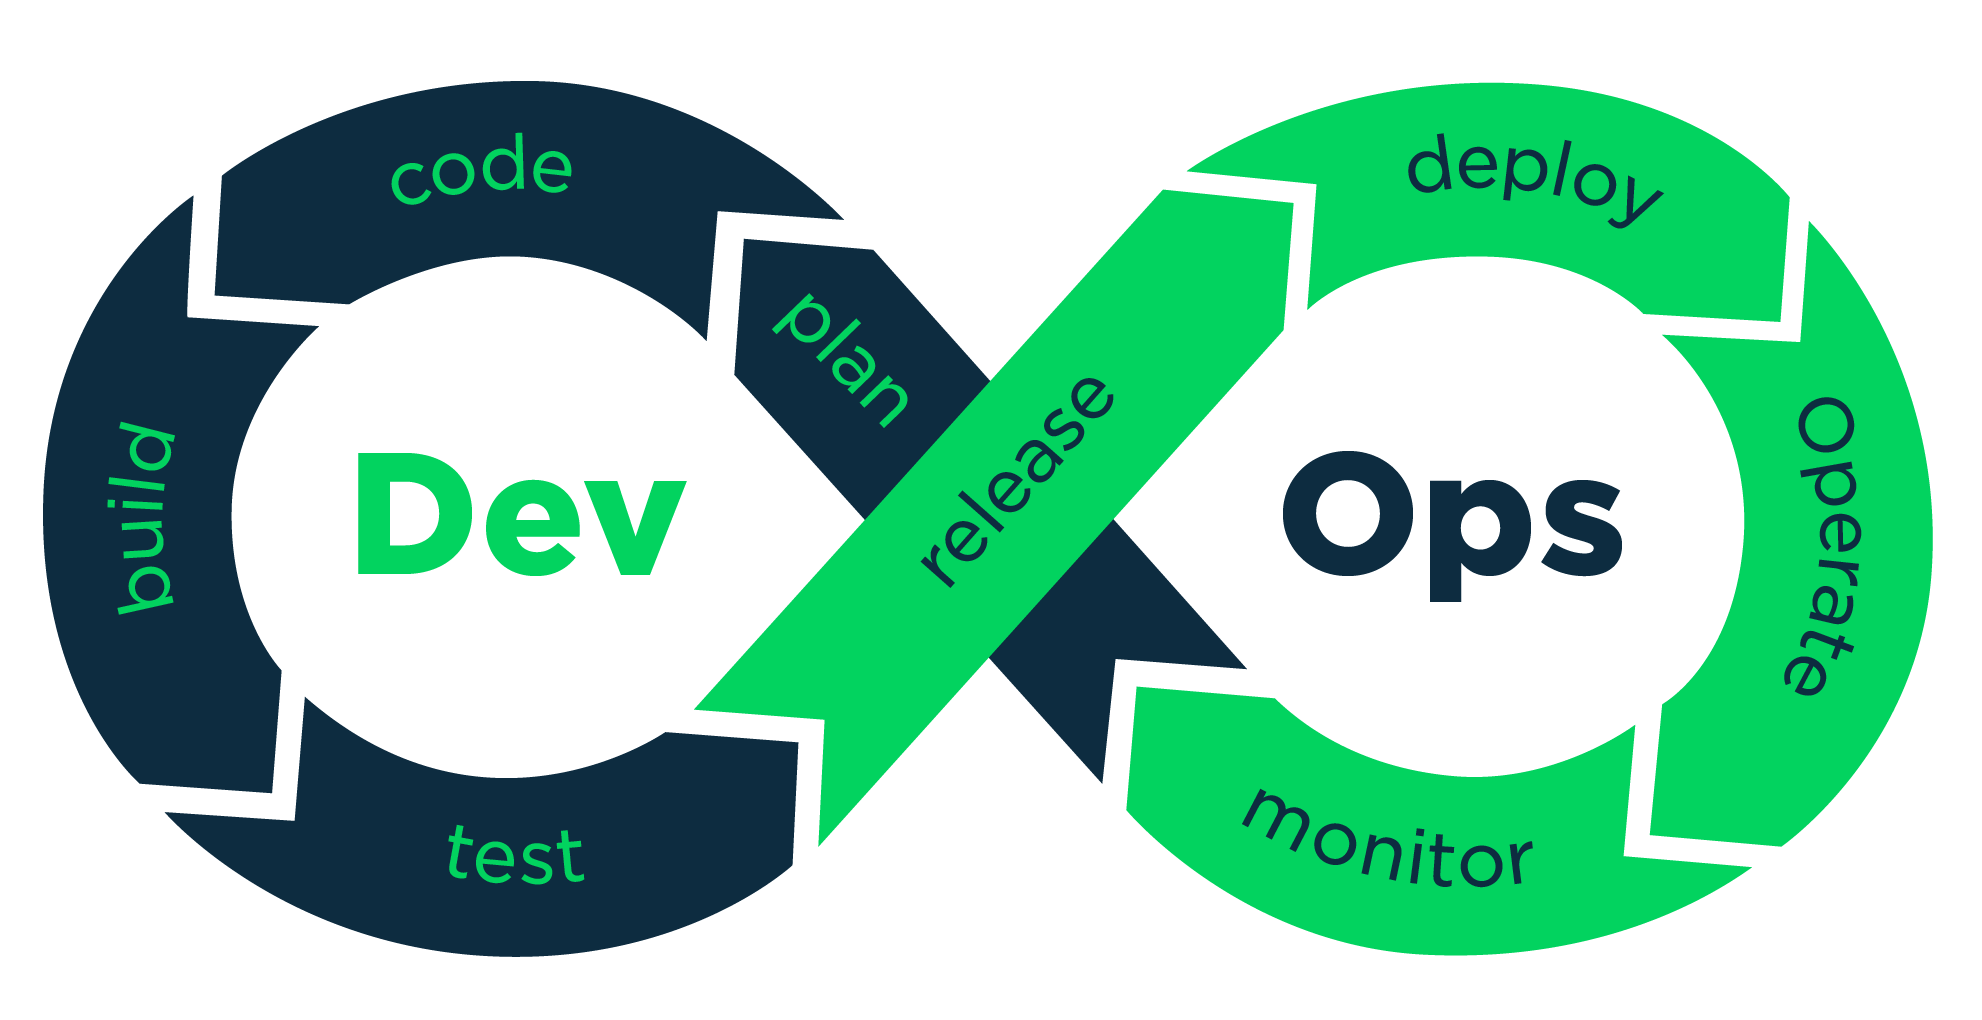
\includegraphics[width=80mm, keepaspectratio]{figures/devops.png}
    \caption{DevOps szemlélet a projektben}
    \label{fig:devops}
\end{figure}
%-----------------------------------------------------------------------------
